\documentclass[border=10pt]{standalone}

\usepackage{tikz}
\usepackage{tikzsymbols}
\usetikzlibrary{calc,patterns,shapes.geometric}

\def\centerarc[#1](#2)(#3:#4:#5){\draw[#1] ($(#2)+({#5*cos(#3)},{#5*sin(#3)})$) arc (#3:#4:#5);}

\begin{document}
	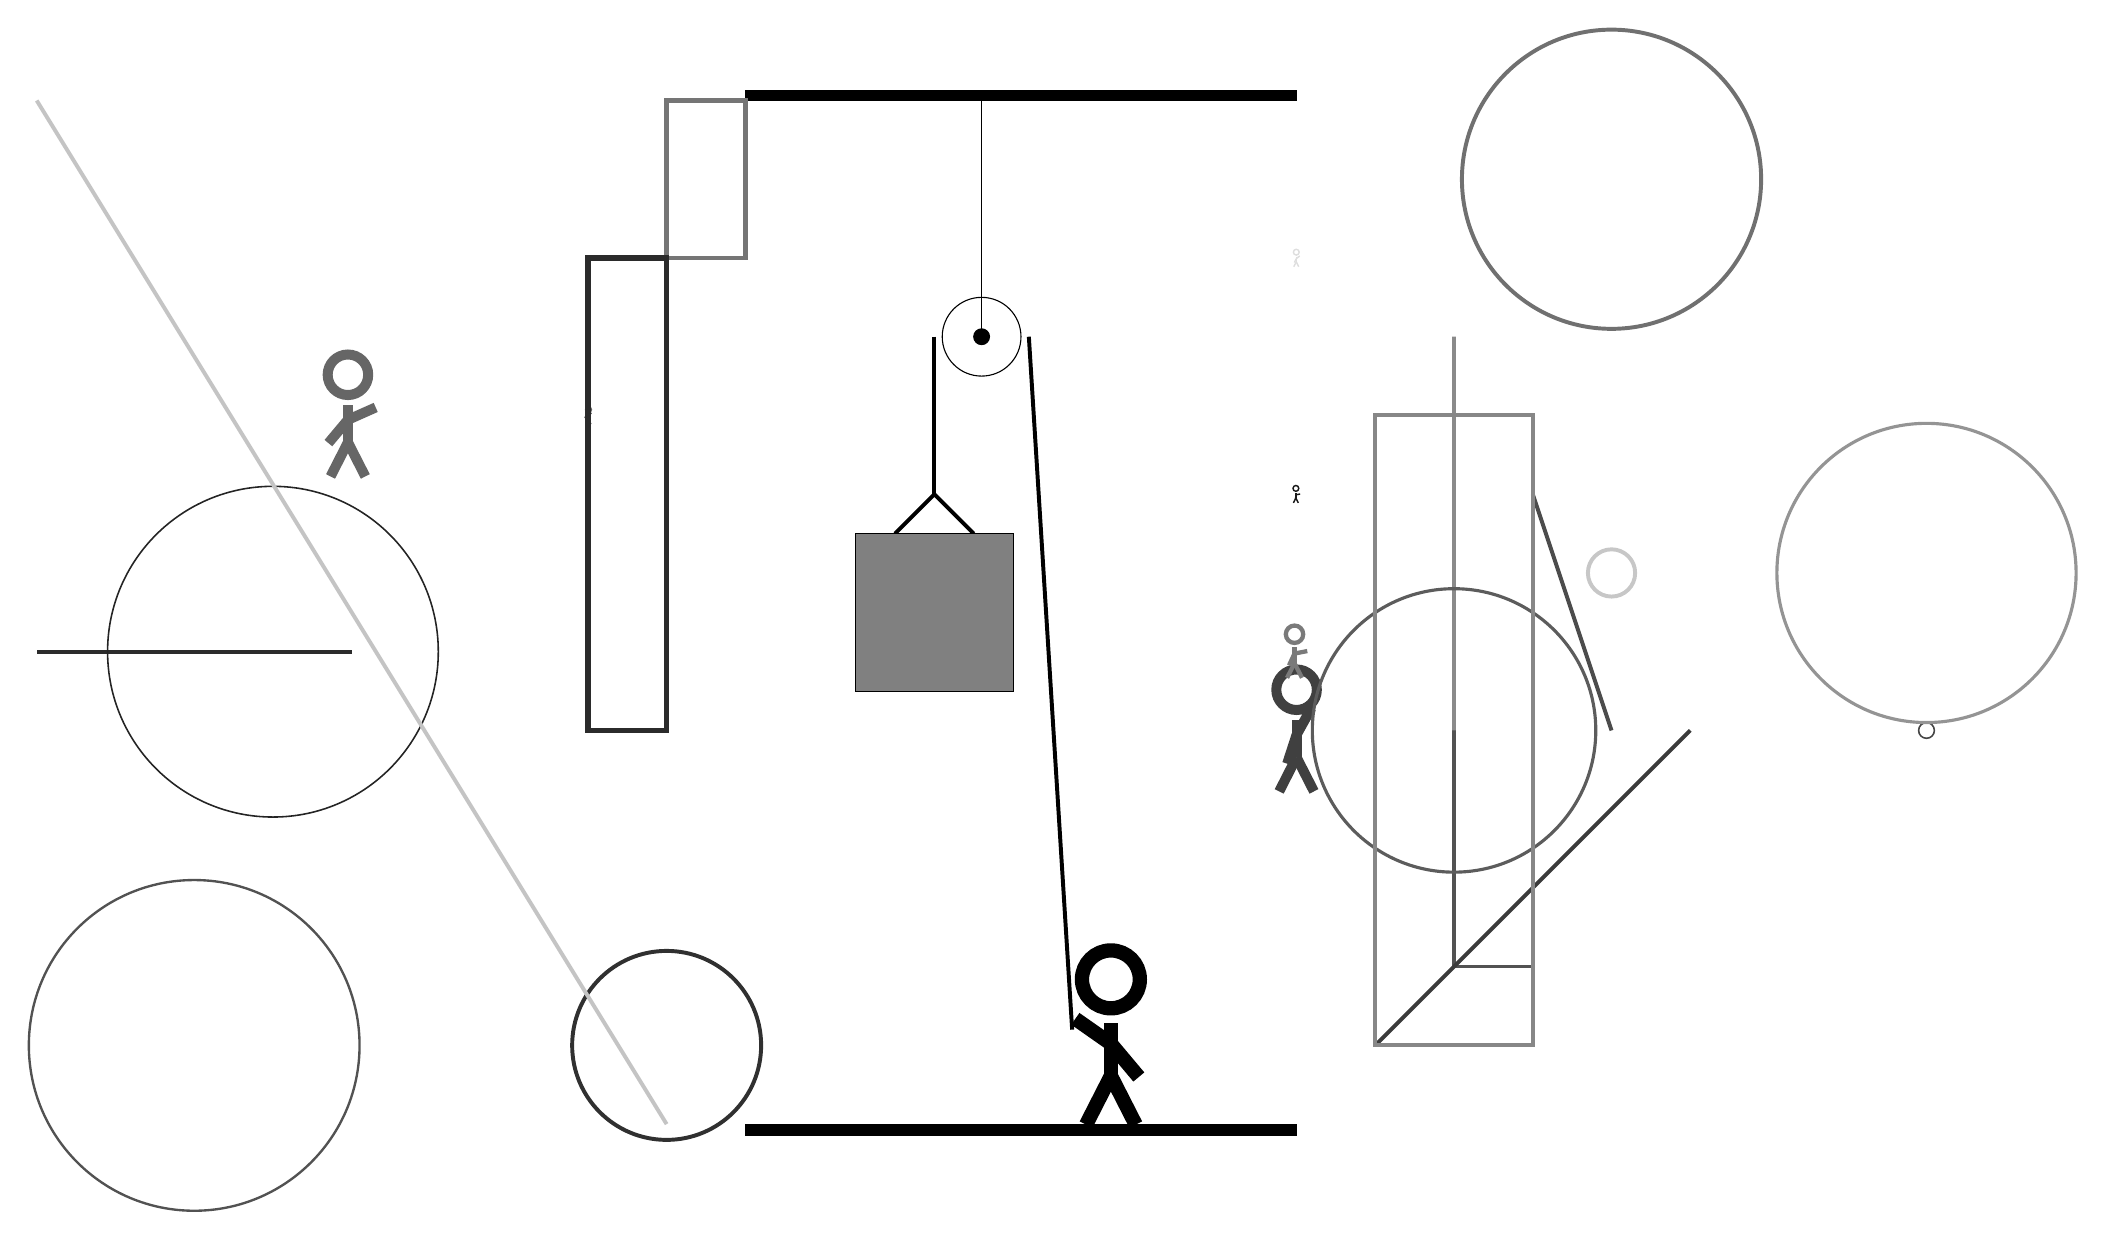
\begin{tikzpicture}
		%%%%% START %%%%%
		
		\draw[fill=black] (-2, 10) rectangle (5, 10.125);
		
		\draw (1, 7) circle (0.5);
		\draw[fill=black] (1, 7) circle (0.1);
		\draw (1, 10) -- (1, 7);
		
		\draw[line width=0.5mm] (-0.1, 4.5) -- (0.4, 5.0) -- (0.9, 4.5);
		\draw[fill=black!50] (-0.6, 4.5) rectangle (1.4, 2.5);
		
		\draw[line width=0.5mm] (0.4, 7) -- (0.4, 5.0);
		\centerarc[line width=0.5mm](1, 7)(0:180:0.6);
		\draw[line width=0.5mm](1.6, 7) -- (2.15, -1.8);
		
		\draw[line width=0.5mm, color=black!83](-7, 3) -- (-11, 3);
		
		\draw[line width=0.4mm, color=black!68] (7, 6) rectangle (8, -1);
		\node[line width=0.7mm, color=black!75] at (5, 2) {\Strichmaxerl[7][72][61]};
		\draw[line width=0.5mm, color=black!46] (7, 7) rectangle (7, 2);
		\draw [line width=0.5mm, color=black!81](-3, -2) circle (1.2);
		\draw [line width=0.5mm, color=black!22](9, 4) circle (0.3);
		\node[line width=0.2mm, color=black!63] at (-4, 6) {\Strichmaxerl[1][19][48]};
		\node[line width=0.7mm, color=black!13] at (5, 8) {\Strichmaxerl[1][64][37]};
		\draw [line width=0.3mm, color=black!68](-9, -2) circle (2.1);
		
		\draw [line width=0.2mm, color=black!86](-8, 3) circle (2.1);
		\draw[line width=0.5mm, color=black!23](-3, -3) -- (-11, 10);
		
		\draw[line width=0.5mm, color=black!70](9, 2) -- (8, 5);
		\draw[line width=0.6mm, color=black!54] (-2, 10) rectangle (-3, 8);
		
		\draw [line width=0.5mm, color=black!56](9, 9) circle (1.9);
		\draw [line width=0.2mm, color=black!73](13, 2) circle (0.1);
		\node[line width=0.4mm, color=black!60] at (-7, 6) {\Strichmaxerl[7][50][24]};
		
		\draw [line width=0.4mm, color=black!64](7, 2) circle (1.8);
		\draw[line width=0.7mm, color=black!83] (-3, 8) rectangle (-4, 2);
		\node[line width=0.3mm, color=black!90] at (5, 5) {\Strichmaxerl[1][86][11]};
		\draw[line width=0.5mm, color=black!77](10, 2) -- (6, -2);
		\draw [line width=0.4mm, color=black!42](13, 4) circle (1.9);
		\draw[line width=0.5mm, color=black!47] (6, 6) rectangle (8, -2);
		
		\node[line width=0.5mm, color=black!52] at (5, 3) {\Strichmaxerl[3][65][11]};
		
		\node at (2.6, -1.9) {\Strichmaxerl[10][-35][-50]};
		
		\draw[fill=black] (-2, -3) rectangle (5, -3.15);
		
		%%%%% END %%%%%
	\end{tikzpicture}
\end{document}